The experimental interface was created with the intention to mimic
clinical practice while generating quantitative inputs for analysis.
Following is the information that the radiologists received before
starting the experiment. Comments on the instructions are provided
in italics and were not seen by subjects.

\subsubsection*{Section 1: Instructions}

You are about to participate in a study on medical decision making.
You may pause the study at any time. To resume, revisit the link you
were given and your progress will have been saved.

We will present you with adult patients with potential thoracic pathologies.
These patients will be presented under the following four scenarios:
\begin{enumerate}
\item Only a chest X-ray is shown.
\item An X-ray is accompanied with additional information about the \uline{clinical
history.}
\item An X-ray is shown along with \uline{Artificial Intelligence (AI)
support}. This AI tool is described in further detail below.
\item An X-ray is shown along with both additional information on \uline{clinical
history} and the \uline{AI support.}
\end{enumerate}
%
The patients are randomly assigned to each of these scenarios. That
is, availability of \uline{clinical history} and/or \uline{AI
support} is unrelated to the patient.

\uline{Clinical History:} includes available lab results or indications
by the treating physician, if any.

\uline{AI support:} This tool uses only the X-ray image to predict
the probability of each potential pathology of interest. The tool
is based on state-of-the-art machine learning algorithms developed
by a leading team of researchers at Stanford University.

\textbf{Responses}

For each patient and pathology, we will ask for both an assessment
and a treatment decision:
\begin{enumerate}
\item We will first ask for your assessment of the probability that each
condition is present in a patient. \textbf{Please consider all pathologies
and findings that would be relevant in a radiology report for the
patient. You should express your uncertainty about the presence of
one or many conditions by appropriately choosing the probability.}
Note that it is possible that the patient has multiple such conditions
or none of them.
\item If you determine that a pathology may be present, we may ask you to
rate the severity and/or extent of the disease on a scale.
\item Finally, when relevant we will ask whether you would recommend treatment
or follow up according to the clinical standard of care if you determine
that the pathology may be present. The first two responses are diagnostic
while the third is a clinical decision. We are aware that a single
physician or radiologist typically does not perform both tasks. However,
for this study, we ask that you respond to the best of your ability
in both of these roles.
\end{enumerate}
\textbf{Browser Compatibility}

This platform supports desktop versions of Chrome, Firefox, and Edge.
Important features on non-supported browsers (including Safari) are
missing and we discourage their use for this experiment. In addition,
the platform does not support any mobile devices and the platform
will perform poorly on mobile. If you encounter any issues during
the experiment, please send an email to \href{mailto:DiagnosticAI@mit.edu}{DiagnosticAI@mit.edu}
and we will follow-up quickly.

\subsubsection*{Section 2: Clinical Hierarchy}

The interface uses a hierarchy to categorize various thoracic conditions.
It will be useful to familiarize yourself with this hierarchy before
you start, but you may also revisit the hierarchy at any time throughout
the experiment by clicking the help tab in the upper right corner.\textit{
{[}The probability for the sub-pathologies is required only if the
parent pathology prevalence is greater than 10\%{]}}

\begin{figure}[H]
\caption{Pathology Hierarchy}

\begin{center}
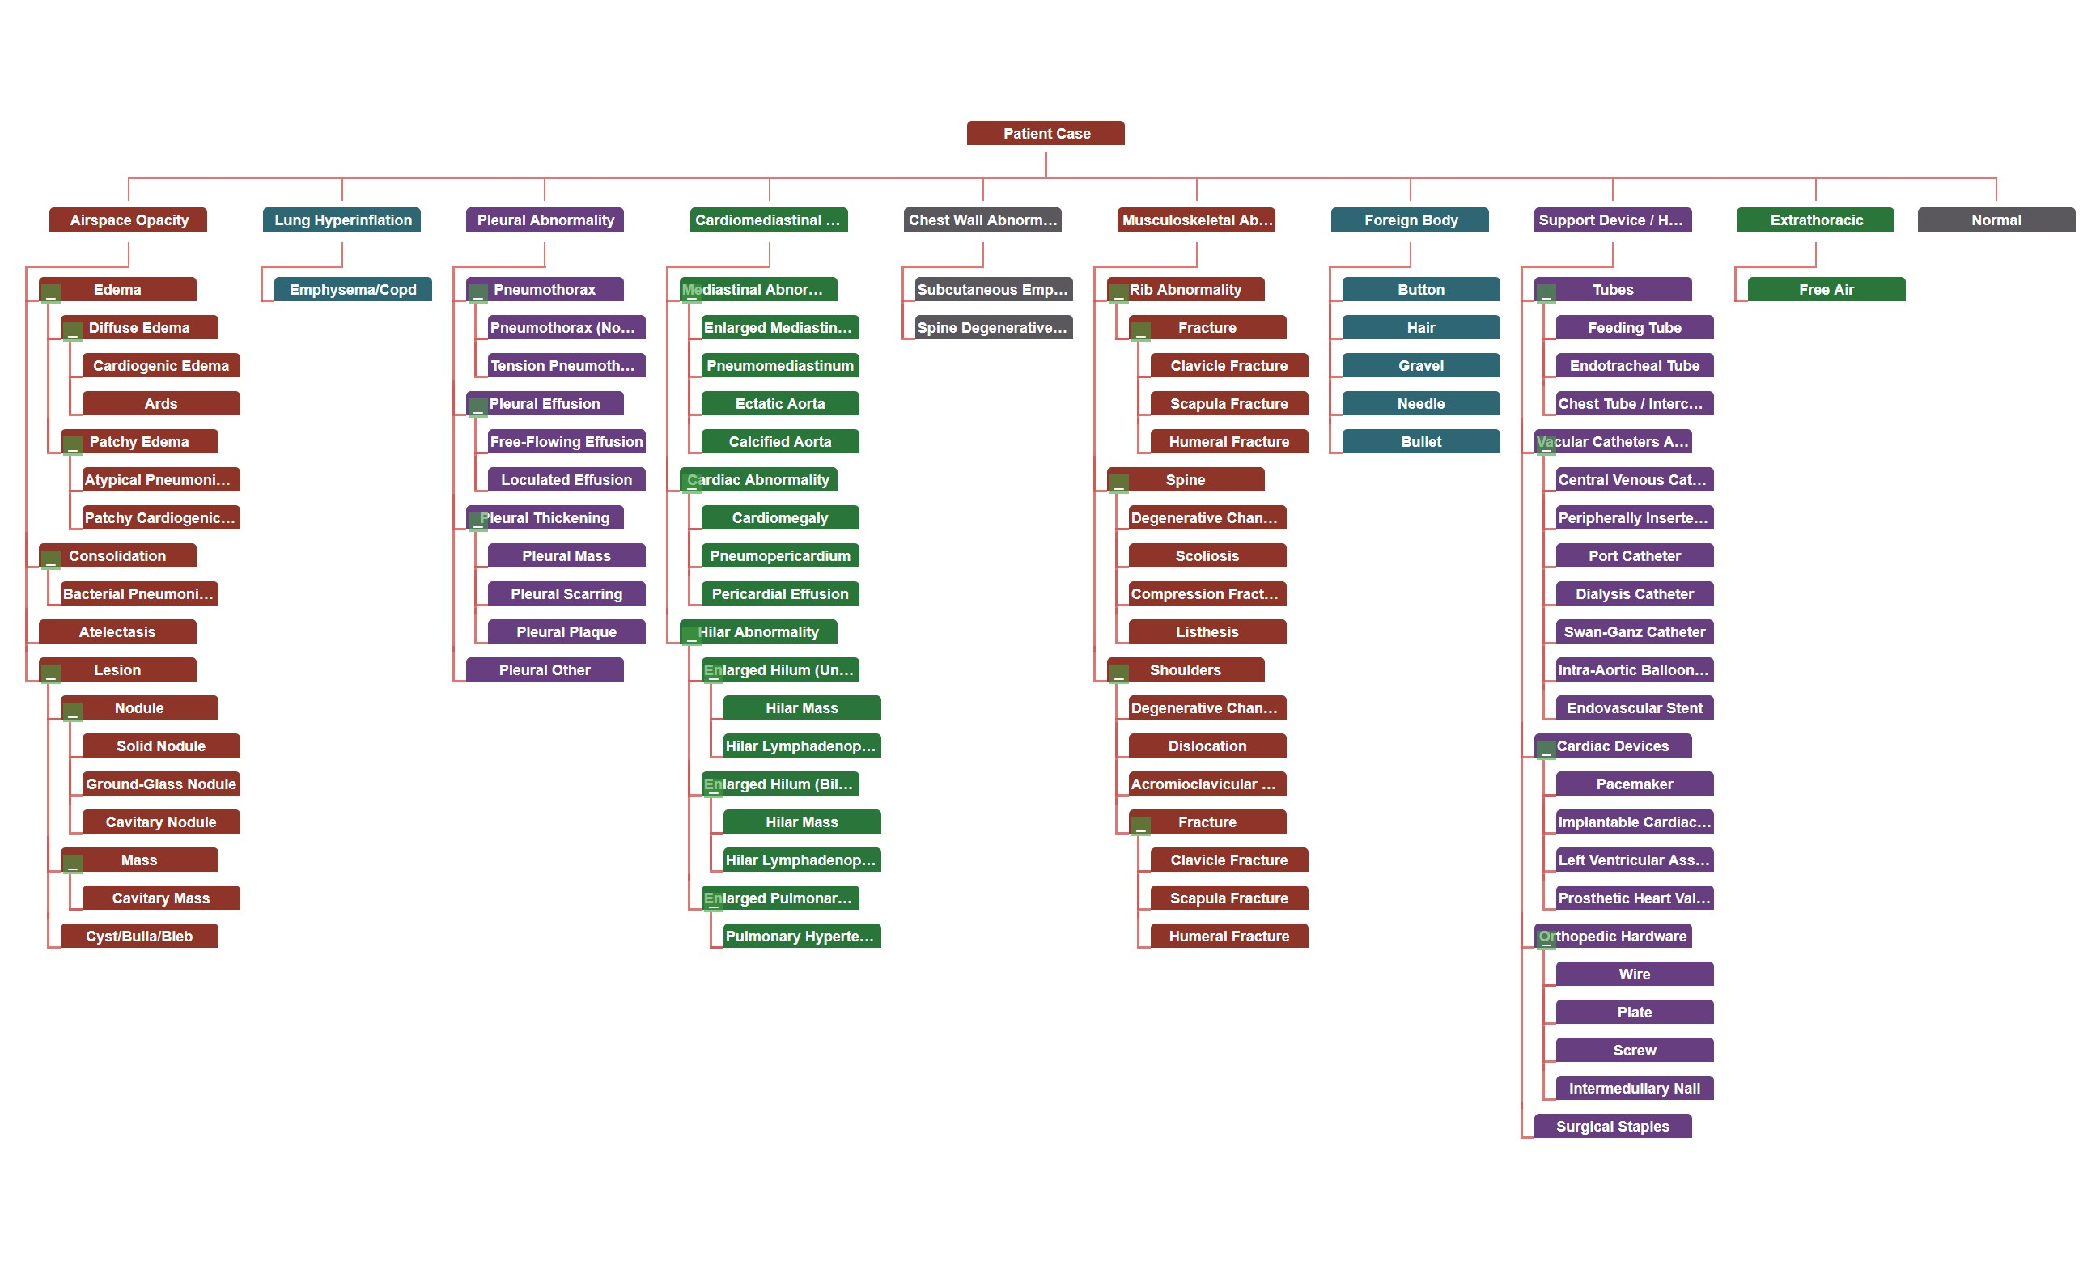
\includegraphics[width=1\textwidth]{images/pat_hierarchy.pdf}
\end{center}
\end{figure}


\subsubsection*{Section 3: AI Support Tool}

The AI support tool that is provided uses only the X-ray image to
predict the probability of each potential pathology of interest. The
tool is based on state-of-the-art machine learning algorithms developed
by a leading team of researchers at Stanford University. The tool
is trained only on X-ray images, meaning it does not incorporate the
clinical history of the patients.

\textbf{Performance of the AI Support}

The AI tool is described in \href{https://arxiv.org/abs/1901.07031}{Irvin et al. [2019]},
which showed the AI tool performed at or near expert levels across
the pathologies studied. Below we plot two measures of performance
of the AI tool. We plot in blue the accuracy of the tool, defined
as the share of cases correctly diagnosed when treating false positives
and false negatives equally. In red, we plot the Area Under the ROC
curve (AUC), which is another measure of AI classification performance.
The AUC is a number between 0 and 100\%, with numbers close to 100\%
representing better algorithm performance. The AUC is equal to the
probability that a randomly chosen positive case is ranked higher
than a randomly chosen negative case.

\begin{figure}[H]
\caption{Performance of AI Tool}

\begin{center}
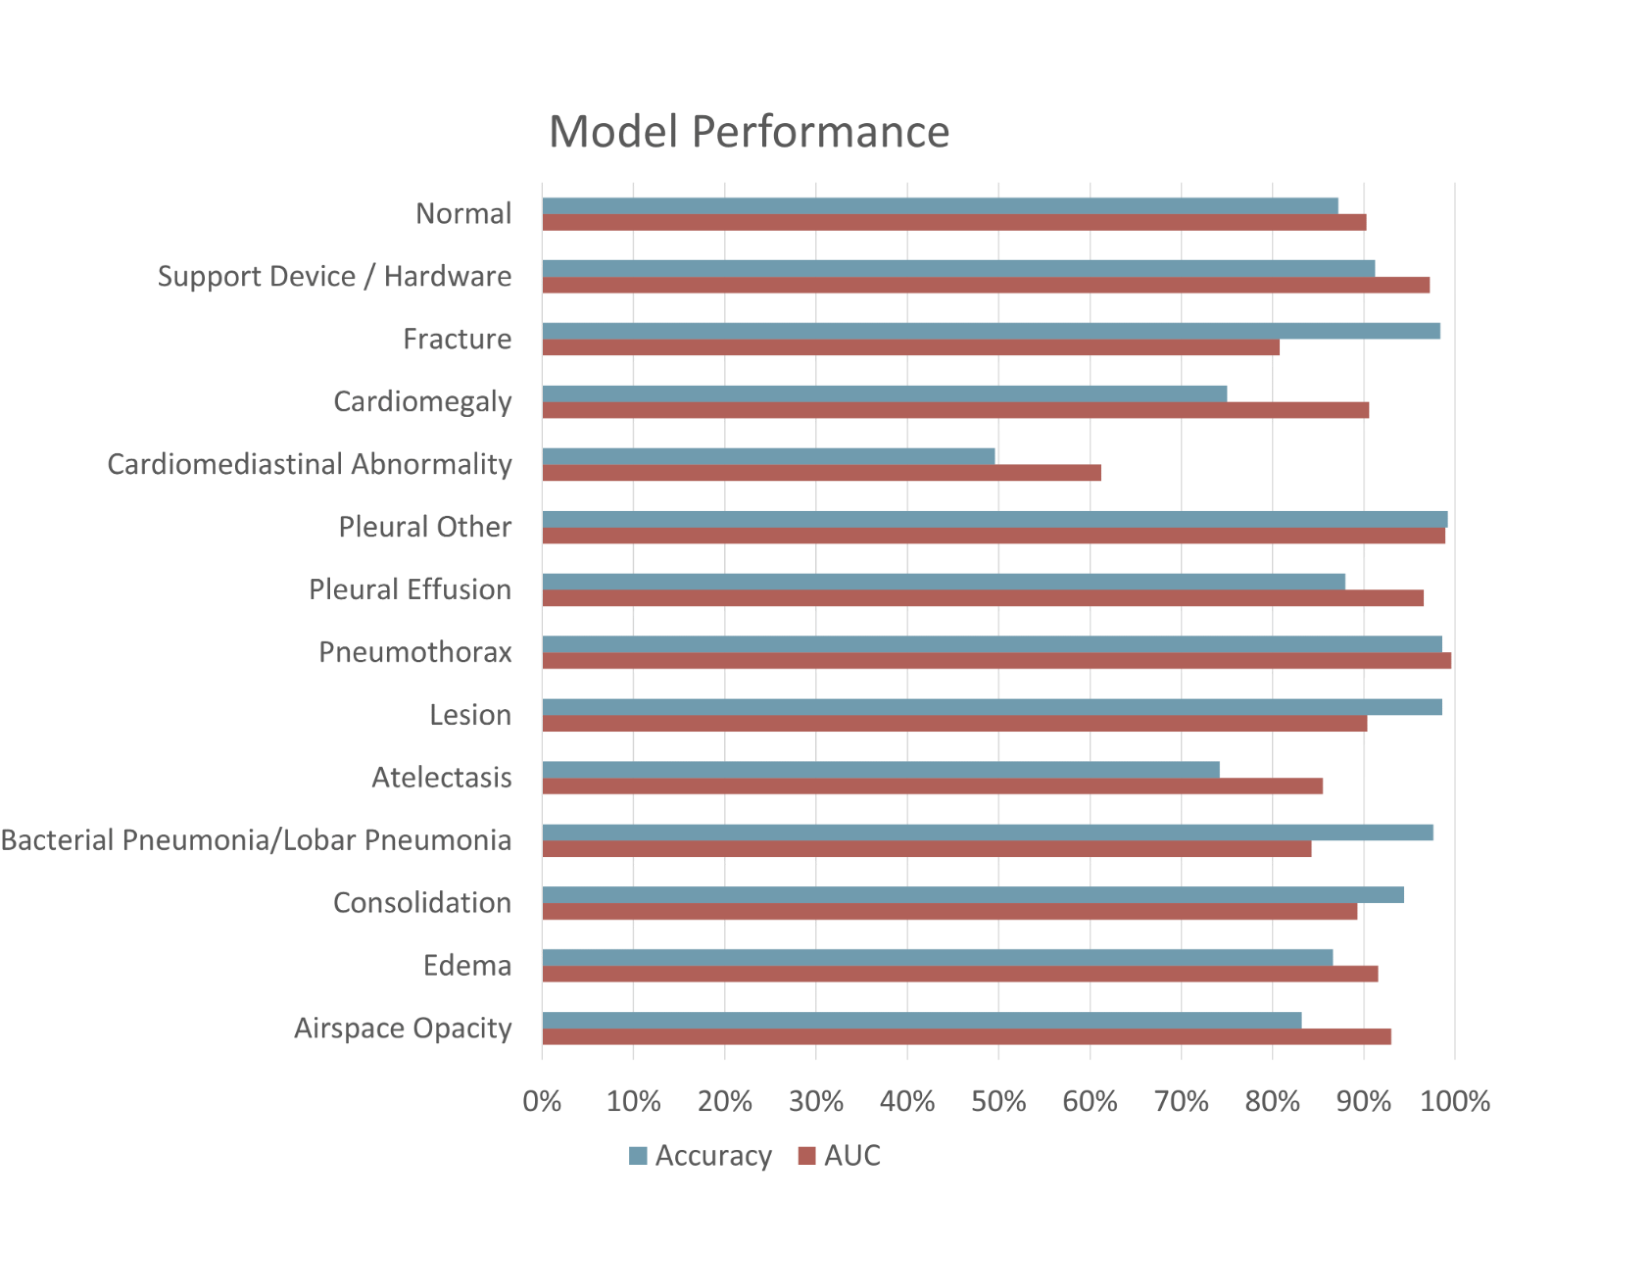
\includegraphics[scale=0.6]{images/ai_instruction_accuracy.pdf}
\end{center}
\end{figure}

\textbf{Example Images}

Below are 50 example images with the associated AI tool predictions.
These images are randomly chosen to allow you to familiarize yourself
with the AI support tool and its accuracy \emph{{[}Here we only provide
two out of the fifty images{]}.}

\begin{figure}[H]
\caption{Example Images}

\begin{center}
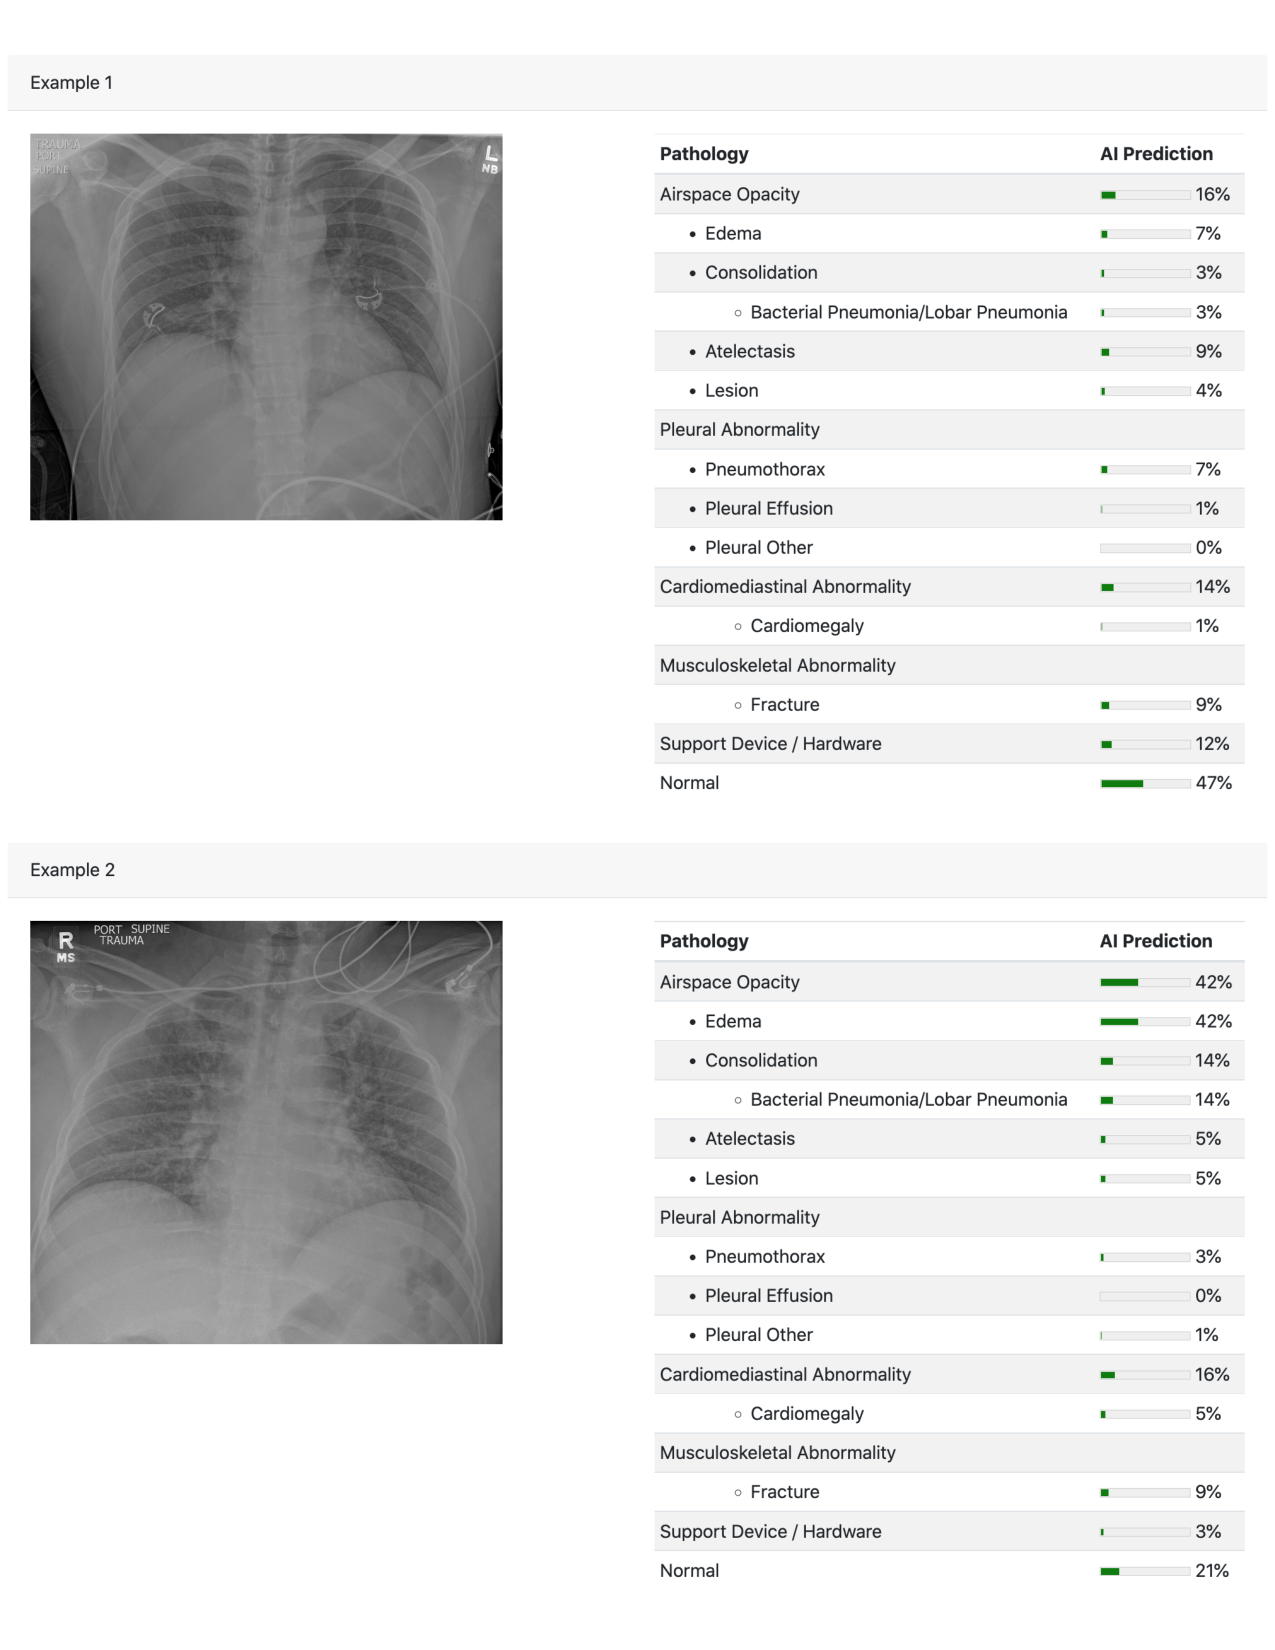
\includegraphics[scale=0.8]{images/ai_instruction_example.pdf}
\end{center}
\end{figure}
\textbf{Section 4: Demonstration}

The brief video below walks you through the interface and a few examples.
\emph{{[}At this stage participants saw an instruction video which
can be founds \href{https://www.dropbox.com/s/fgdcokweekpm44r/RadExperimentV4.mp4?raw=1}{here}{]}}

\subsubsection*{Section 5: Consent I}

You have been asked to participate in a study conducted by researchers
from the Massachusetts Institute of Technology (M.I.T.) and Harvard
University.

The information below provides a summary of the research. Your participation
in this research is voluntary and you can withdraw at any time.
\begin{enumerate}
\item Study procedure: We will ask you to examine a number of chest x-rays.
We will vary both the amount of information provided about the patient
and the availability of an AI support tool.
\item Potential Risks \& Benefits: There are no foreseeable risks associated
with this study and you will receive no direct benefit from participating.
\end{enumerate}
%
Your participation in this study is completely voluntary and you are
free to choose whether to be in it or not. If you choose to be in
this study, you may subsequently withdraw from it at any time without
penalty or consequences of any kind. The investigator may withdraw
you from this research if circumstances arise.

\subsubsection*{Section 6: Consent II}

\textbf{Privacy \& Confidentiality}

The only people who will know that you are a research subject are
members of the research team which might include outside collaborators
not affiliated with MIT. No identifiable information about you, or
provided by you during the research, will be disclosed to others without
your written permission, except: if necessary to protect your rights
or welfare, or if required by law. In addition, your information may
be reviewed by authorized MIT representatives to ensure compliance
with MIT policies and procedures.

When the results of the research are published or discussed in conferences,
no information will be included that would reveal your identity.

\textbf{Questions}

If you have any questions or concerns about the research, please feel
free to contact us directly at diagnosticAI@mit.edu.

\textbf{Your Rights}

You are not waiving any legal claims, rights or remedies because of
your participation in this research study. If you feel you have been
treated unfairly, or you have questions regarding your rights as a
research subject, you may contact the Chairman of the Committee on
the Use of Humans as Experimental Subjects, M.I.T., Room E25-143B,
77 Massachusetts Ave, Cambridge, MA 02139, phone 1-617-253 6787.

I understand the procedures described above. By clicking next, I am
acknowledging my questions have been answered to my satisfaction,
and I agree to participate in this study.

\subsubsection*{Section 7: Interface questions}

\emph{{[}Each of these questions has a true of false response which
was entered through a radio button. Participants are not able to start
the experiment without answering each question correctly.{]}}

Before beginning the experiment, we would like to confirm a few facts
through the following comprehension questions. Please answer True
or False to the following questions.

1) The algorithm's prediction is based on information from both the
X-ray scan as well as the clinical history.

2) When the algorithm does not show a prediction, it is because the
algorithm thinks the pathology is not present.

3) The follow up decision refers to any treatment or additional diagnostic
procedures that one would conduct based on the findings of the report.

4) Two patients with the same probability score for a condition ought
to always receive the same \textquotedblleft follow-up\textquotedblright{}
recommendation.

5) When a condition at a higher level of the hierarchy receives a
less than ten percent chance of being present then all the lower level
conditions within this branch automatically receive a zero probability
of being present.

6) If the algorithm says that the probability of a pathology is present
with 80\% probability, it means that the AI predicts 80 cases out
of 100 have the pathology present.

7) Suppose your assessment is that the patient definitely has either
edema or consolidation, and you believe that edema is twice as likely
as consolidation. Then you would assign 66.67\% to edema and 33.33\%
to consolidation:

8) I should only indicate pathologies and findings that would be relevant
in a radiology report for the patient.

\subsubsection*{Section 8: Bonus (Randomized only for designs 1 and 3)}

Bonus Payment Thank you again for participating in our study. If your
responses in this section are close to the average response of an
independent group of radiologists for each case, we will give you
a \$120 gift card to a large e-commerce retailer of your choice (e.g.
Amazon, Flipkart). This payment rule is designed so that your chances
of winning the prize is highest if you report your best estimate of
the probability that the pathology is present. The precise payment
rule is available on request, and we will follow up after the experiment
if you win the gift card.

\subsubsection*{Section 9: Practice Images}

First, we will present you with 8 patients (Design 1) to practice
and familiarize yourself with the interface. In the practice you will
see 2 patient cases under each of the possible combinations of AI
support and clinical history availability. You will be compensated
for these reads even though they are just for practice. {[}\textit{5
practice images for design 1 and none for design 3}{]}

\subsubsection*{Section 10: Randomized Information Scenario }

{[}\textit{This is the start of the experiment. The dataset contains
only these observations and excludes any practice images data.}{]}

The extent of clinical history information provided is not homogenous.
The thoroughness of the information varies across available information
for every patient. Some examples of varying clinical history information
are: 


